\section{Training and performance evaluation} %2-3 pages
%
%- Performance metrics: training time, inference time
%- energy consumption
%
Over the whole project we stuck to the dataset of 1000 images of each class, split into 80\% training, 20\% testing using the function \code{get\_data} with the randomness seed ``1550'', our results are reproducible.
%One epoch has passed when each of the training images has been used once for the training.
The used parameters and results of the given tests can be retrieved from the JSON files in the results folder.

\subsection{Linear Regression}
As a baseline to compare our optical machine learning model against, a linear regression is performed.
The results of the linear regression with and without energy normalization and for different values of the image side-lengths ($m=[1,2,4,6,8,10,16,20,28]$) are compared. 
\begin{wrapfigure}{r}{7cm}
%\begin{figure}[H]
    \centering
    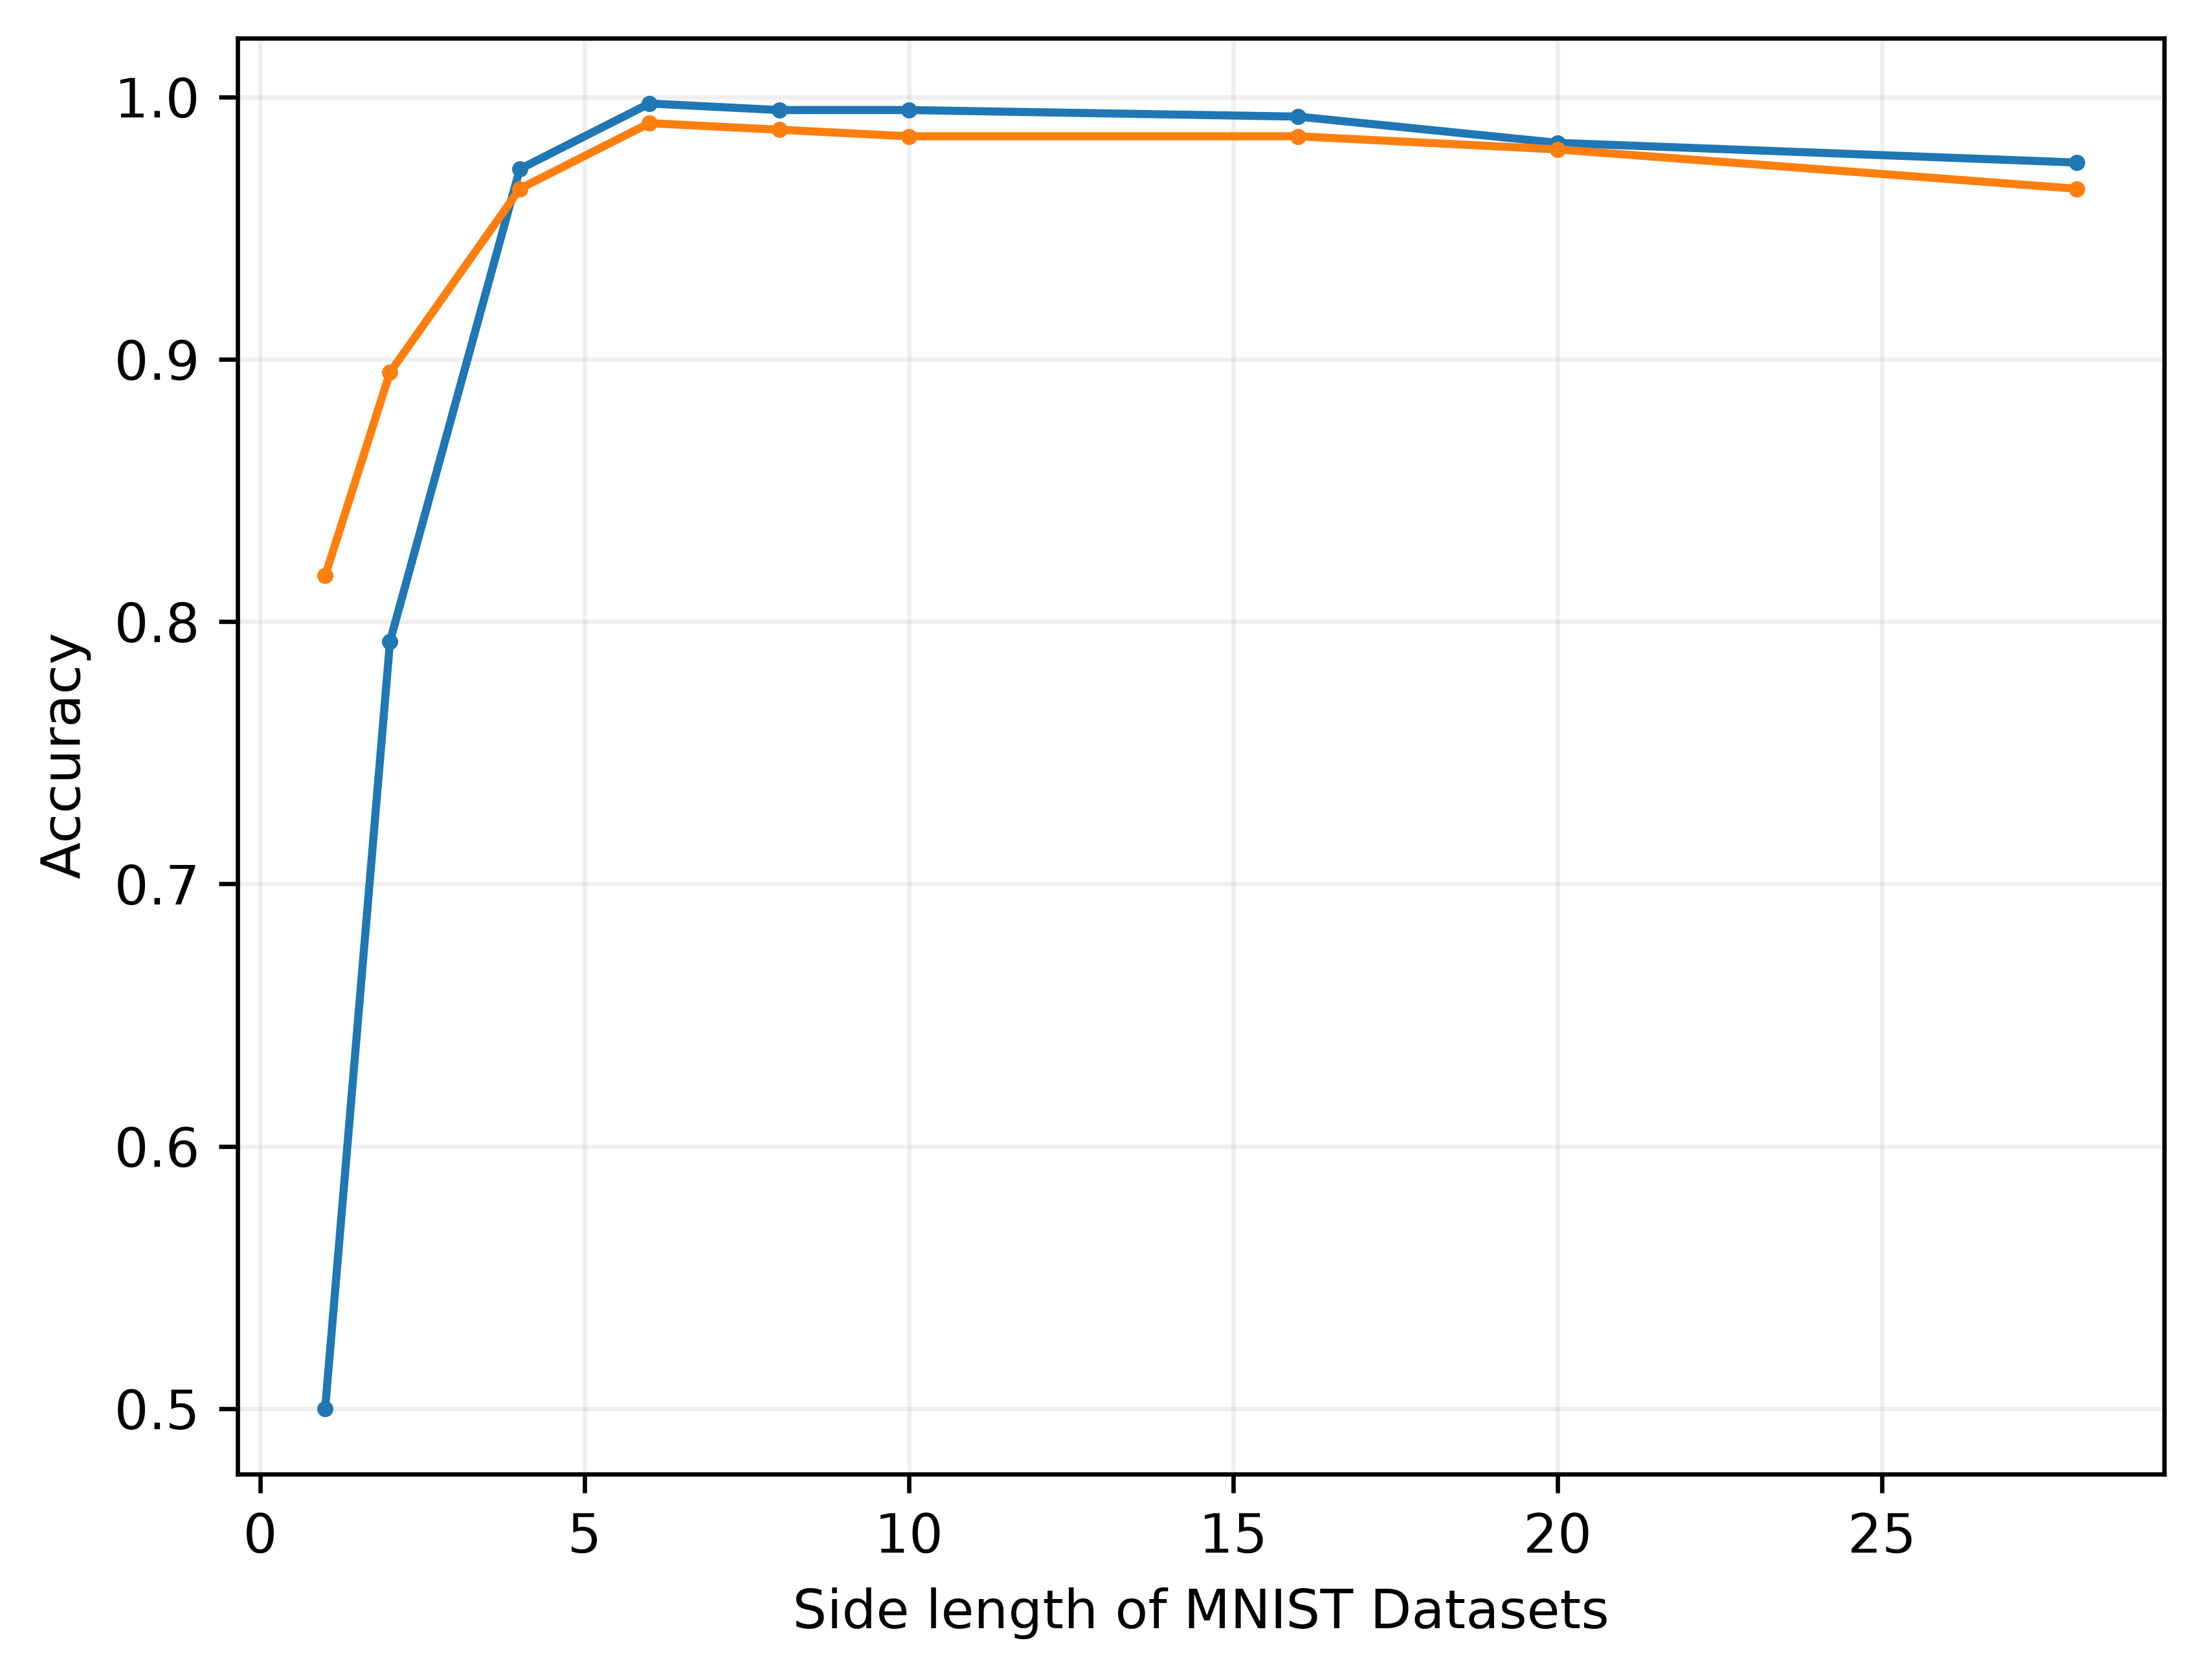
\includegraphics[width=0.9\linewidth]{evaluation/linear_regression/m_sweep_with_and_without_energy_normalization.png}
    \caption{Accuracy of the linear regression with (blue graph) and without (orange graph) energy normalization for different side lengths of the images.}
    \label{fig:linear_regression_m_sweep}
%\end{figure}
\end{wrapfigure}
A side-length of $m=6$\,px with energy normalization yields the highest testing accuracy with a value of 0.998.
For all m-values except $m=1$ and $m=2$, the energy normalization method yields better results.
The superior performance of the non-normalized case for these low m parameters is explained by the fact, that all of the information of the picture is contained in only one and 4 pixel respectively.
In this case, the model is basically trained on the ``used ink'' to draw the digit. This is also the reason why the energy-normalized mode performs better for larger m. If more information-carrying features are available, the information about overall energy in the system is more prone to generate confusion, for example due to a thicker written ``1''.
The high accuracy of the linear regression shows, that the given classifying problem is almost linearly separable. 

\subsection{Initialization of mesh's phase shift parameters and layer number}
\label{ssec:MeshInit}
The behavior and performance of our model is examined for the two different initialization methods.
In Figure \ref{fig:Mesh_Init_Random_and_Haar}, the intensities of an electric field at input port 50 are visualized.
It is visible that for the Haar initialization, the electric field reaches the edges of the mesh much faster than for the random initialization.
\begin{figure}[H]
    \centering
    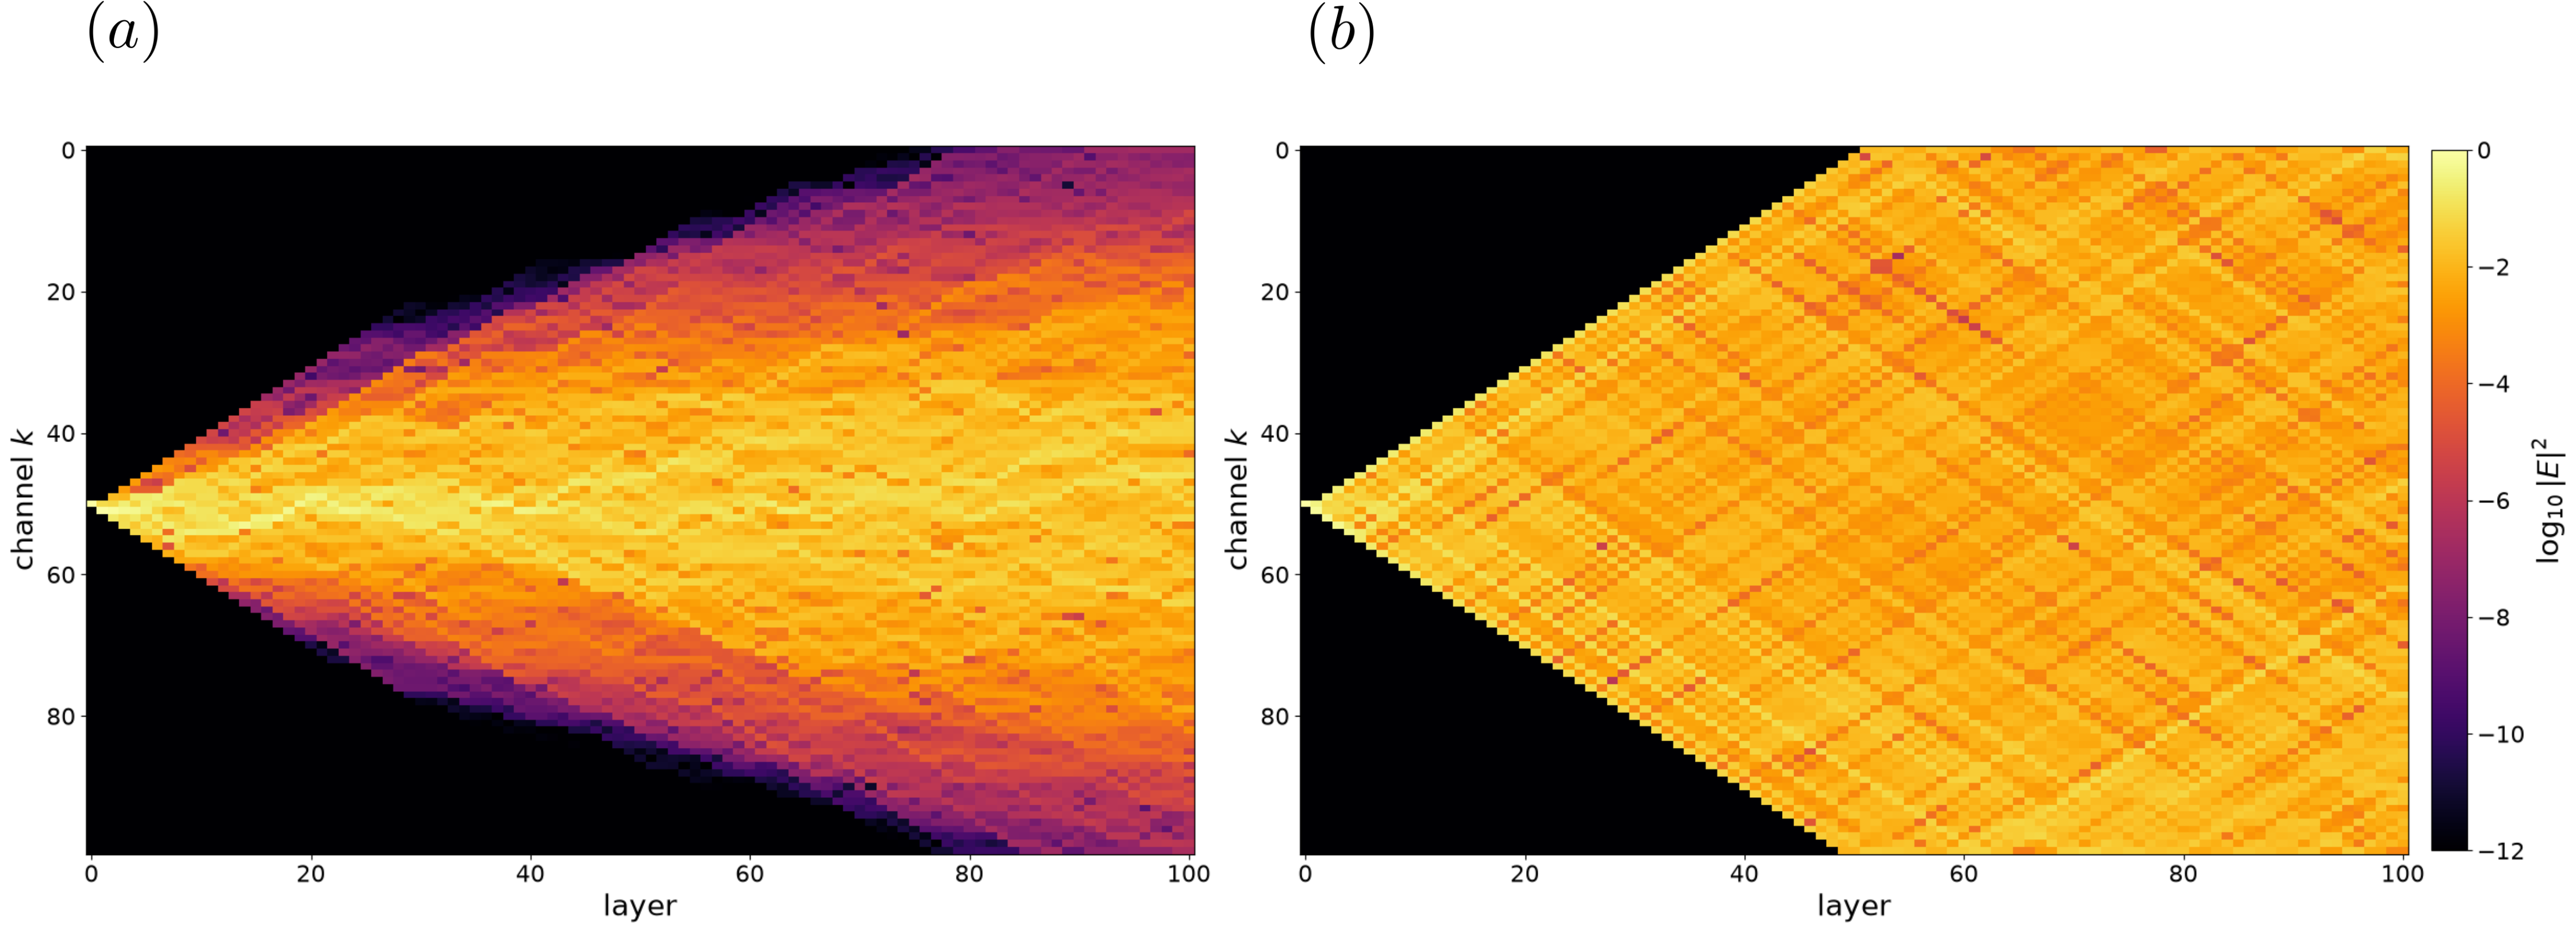
\includegraphics[width=0.8\linewidth]{evaluation/initialization/initComparisson.png}
    \caption{Intensity plot of a normalized electric field starting from channel 50. The mesh's parameters are initialized according to (a) uniform initialization, (b) Haar initialization for uniformly random global transfer matrices.}
    \label{fig:Mesh_Init_Random_and_Haar}
\end{figure}
The training and test results are shown in Figure \ref{fig:init_sweep}.
The training loss of the Haar initialization decreases faster than for the random initialization, leading to a faster convergence.
The random initialization reaches a training accuracy of 0.958 after 29 epochs or 355\,s. The testing accuracy is 0.980.
The Haar initialization reaches a training accuracy of 0.958 after 16 epochs or 185\,s, while the testing accuracy is 0.970.
\begin{figure}[H]
    \centering
    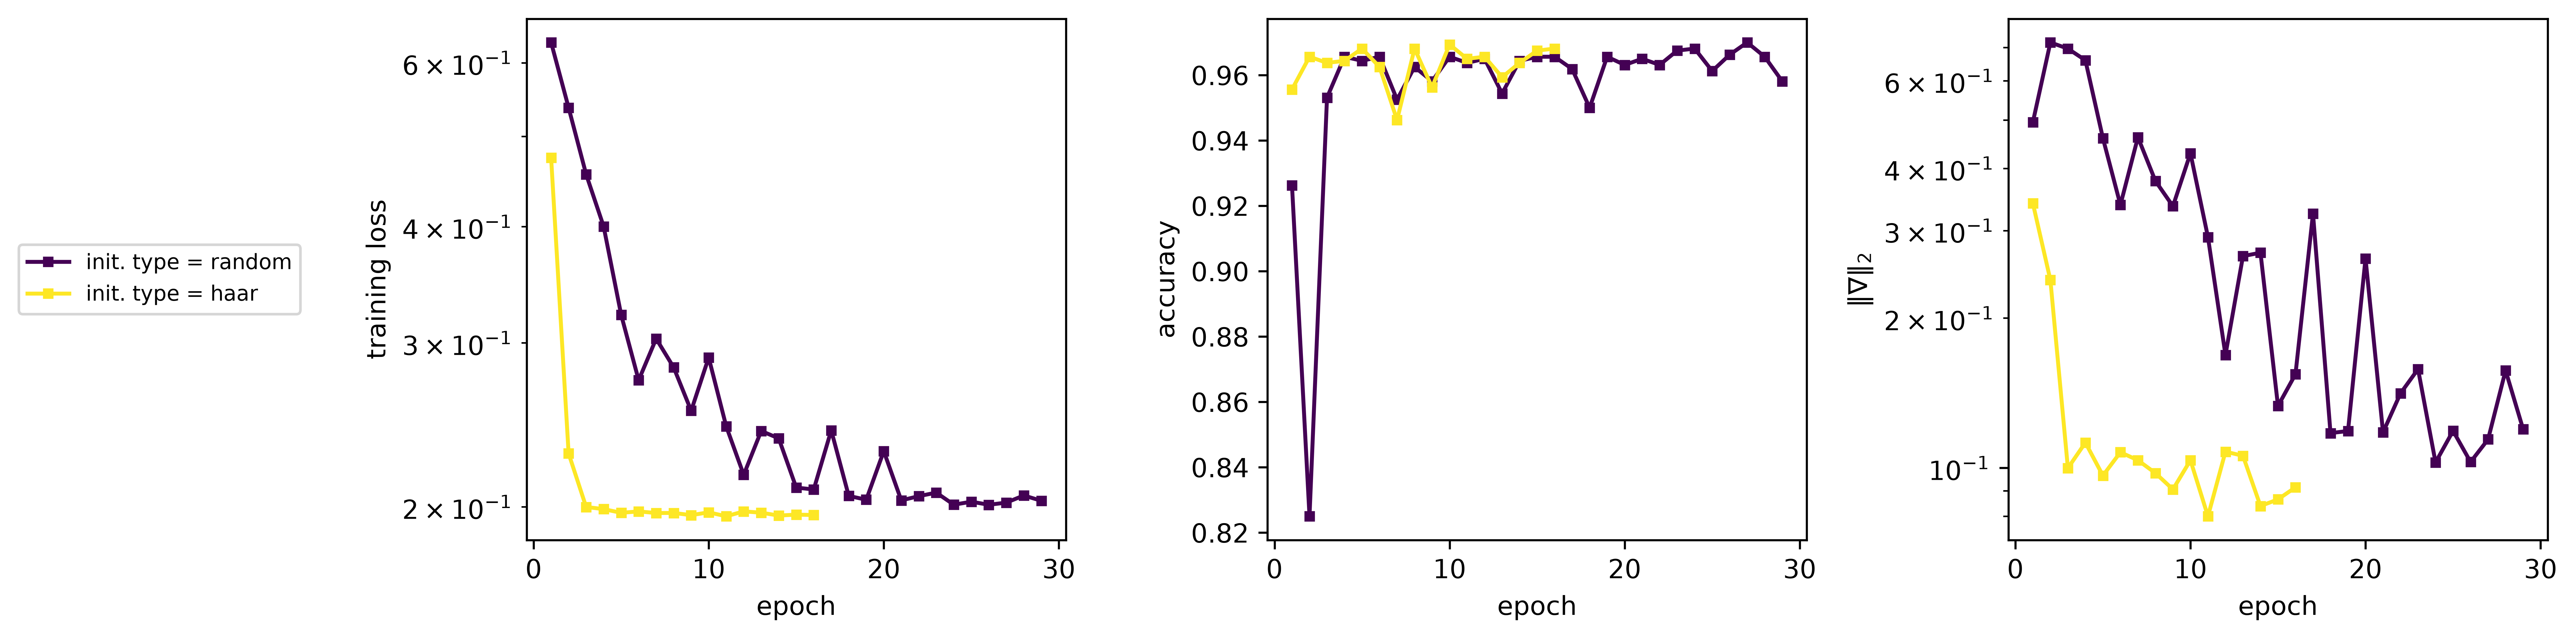
\includegraphics[width=\linewidth]{evaluation/initialization/plot_training_epoch.png}
    \caption{Training loss, training accuracy and normalized gradient for random and Haar initialization.}
    \label{fig:init_sweep}
\end{figure}
%init. type=random  epochs= 29 loss=0.20297  train acc=0.9581  test acc=0.9800  355s
%init. type=haar  epochs= 16 loss=0.19596  train acc=0.9681  test acc=0.9700  185s

%\subsection{Layer number}
To see impact of different \gls{mzi} meshes with respect to the layer number, we perform training over different values. Since the haar initialization promises for faster mixing of the signal inside the mesh over random initialization, we perform this training for both.
For Haar initialization, the performance of our model for different numbers of layers in the \gls{mzi} mesh is shown in Figure \ref{fig:layer_count_sweep}.
The training loss decreases most for the layer counts of 100 and 150, and least for the lowest layer count of 10. The training loss for 200 layers behaves similar to the next lower examined layer counts, but is slightly higher.
The training accuracy is highest for the layer counts of 100, 150 and 200.
For the random initialization, see Figure \ref{fig:layer_count_sweep_random_init}, the relative performance is equivalent with higher layer counts converging faster and yielding higher accuracies. Compared to the previous initialization however, the slower convergence becomes clearly visible for all layer sizes. Also the maximum achieved testing accuracy with 0.968 is subordinate to the value of 0.975 of the Haar initialization.
Since less layers mean a less complex physical setup and consequently less losses, the Haar initialization allows a smaller setup.

\begin{figure}[H]
    \centering
    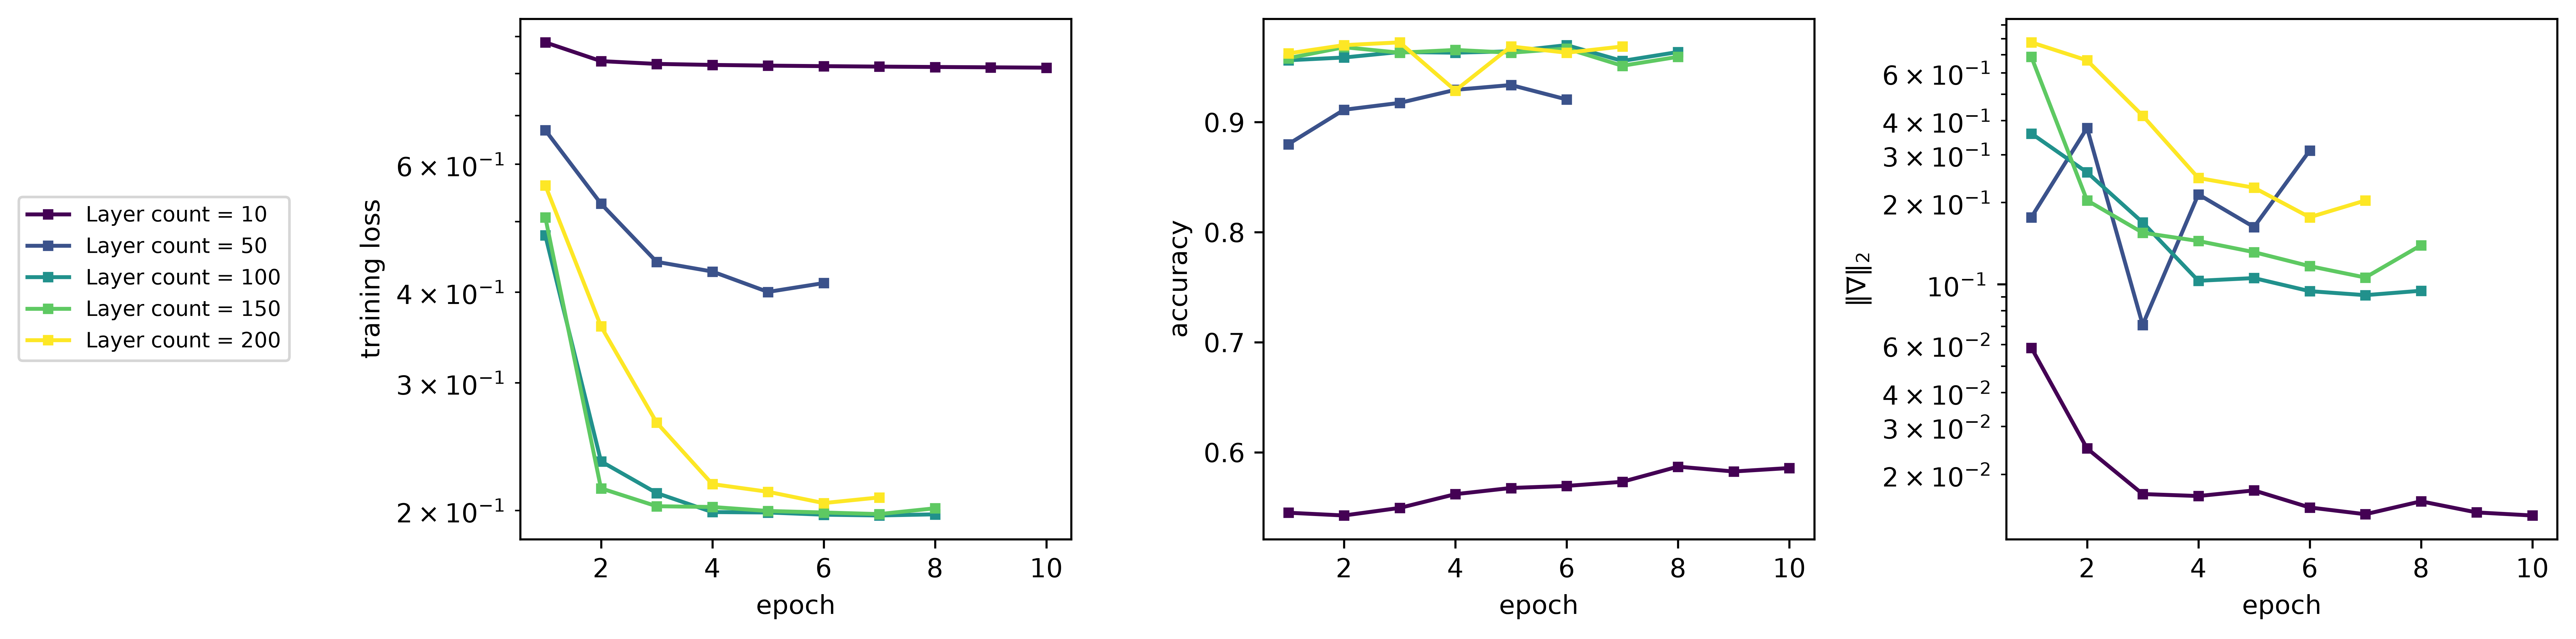
\includegraphics[width=1\linewidth]{evaluation/layer_count/plot_training_epoch.png}
    \caption{Training loss, training accuracy and normalized gradient for different numbers of layers with Haar initialization.}
    \label{fig:layer_count_sweep}
\end{figure}

\begin{figure}[H]
    \centering
    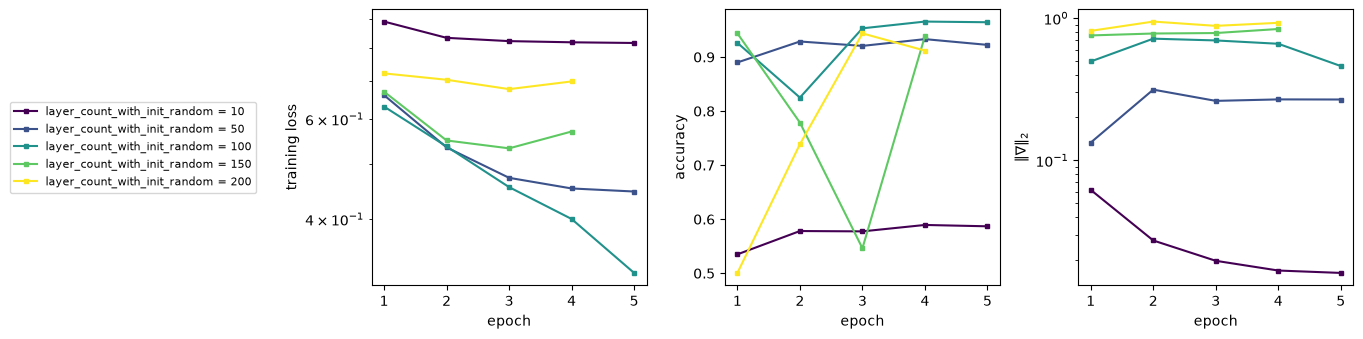
\includegraphics[width=1\linewidth]{evaluation/layer_count/plot_training_epoch_random_init.png}
    \caption{Training loss, training accuracy and normalized gradient for different numbers of layers with random initialization.}
    \label{fig:layer_count_sweep_random_init}
\end{figure}


\subsection{Learning rate analysis}
Sweeping over different learning rates is performed to see the effect on the convergence speed and the achieved accuracy.
We limit the runtime by using a patience value of 5 and a \code{min\_delta=1e-4}. Therefore, we make sure not to waste training time when no further improvement or no convergence at all is possible.
We run it over three different batch sizes (256, 64 and 4). We begin by using 64 to find the best performing learning rate (see Fig. \ref{fig:learning_rate_medium_batch_sweep}) and use 256 and 4 (see appendix \ref{appendix:graph-learningrate}) to see how this optimal learning rate differs based on batch sizes.

The highest learning rates converge fast but reach only a low training accuracy.
It is clearly visible how lower learning rates lead to a slower but more stable convergence. 
This behavior is confirmed for all three tested batch sizes.
Based on the results, a reasonable trade-off seems to be reached for learning rates of 1.0 to 1.7.
\begin{figure}[H]
    \centering
    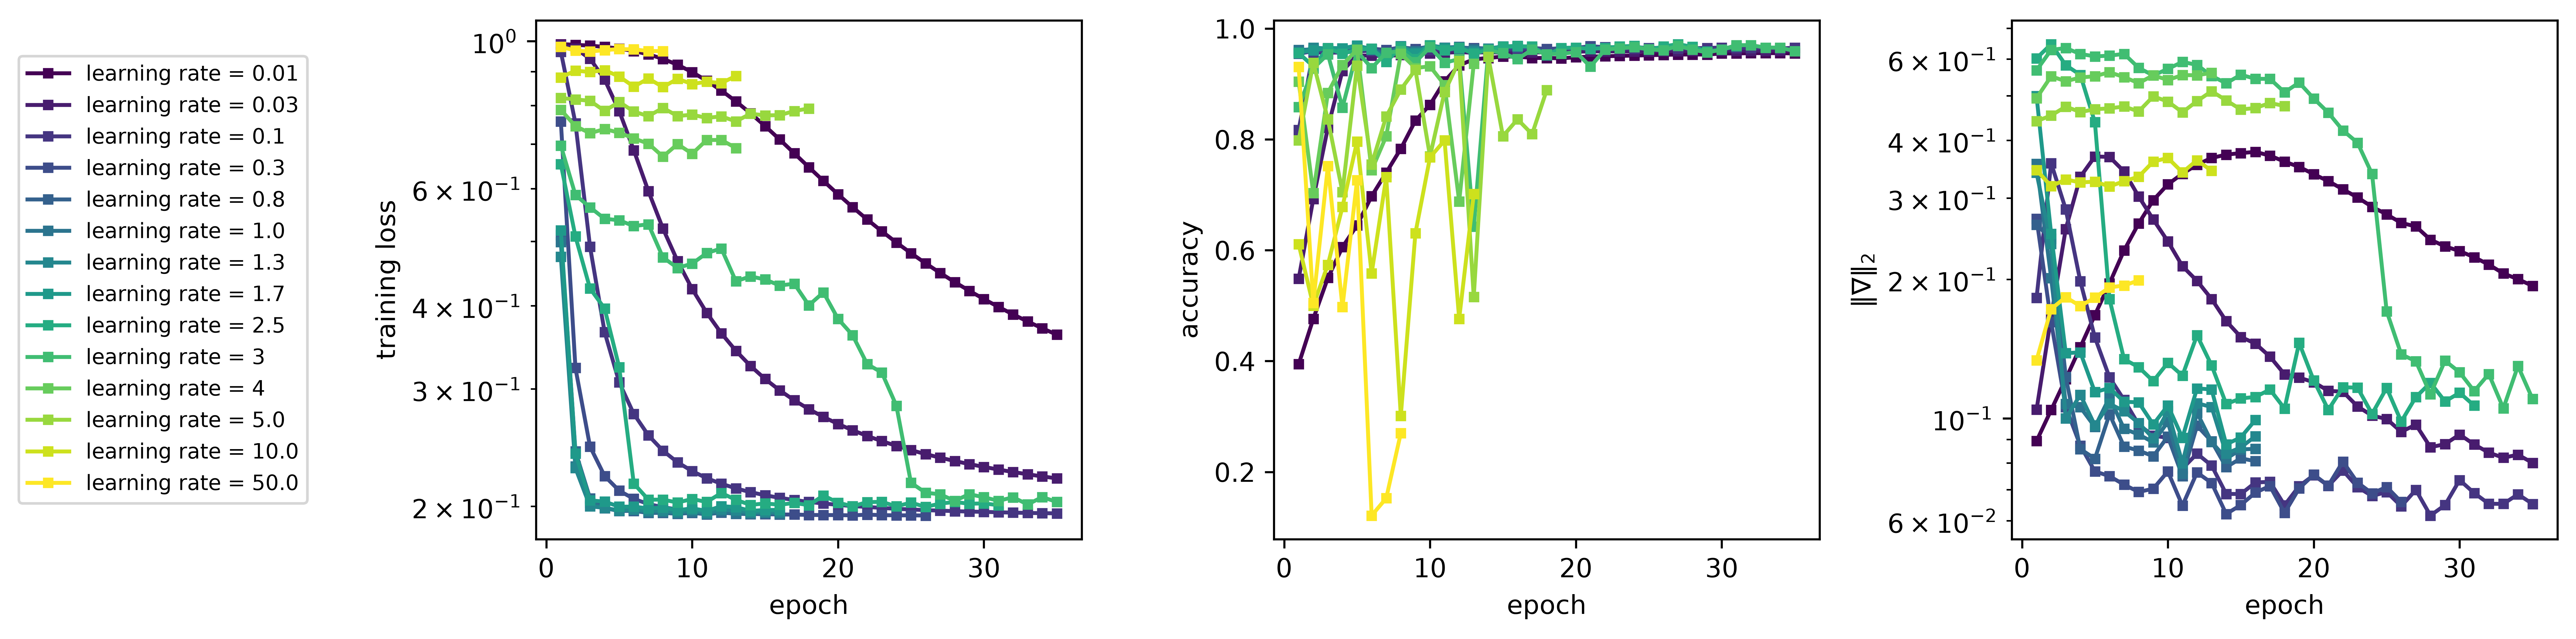
\includegraphics[width=1\linewidth]{evaluation/learning_rate/64_plot_training_epoch.png}
    \caption{Training loss, training accuracy and normalized gradient for different learning rates for a batch size of 64.}
    \label{fig:learning_rate_medium_batch_sweep}
\end{figure}

%Interestingly, the gradient norm for the lowest learning rate is increasing first, until reaching a maximum and the decreasing. 
%Hier außerdem ganz interessant, dass man bei der gradienten Norm sieht, wie die langsame Kurve wohl eine Verringerung des losses erreicht, in dem sie zunächst durch die loss landschaft wandert, wo die gesamte gradienten norm (da gibts so ein Wort) erstmal zunimmt, aber da halt die "wichtigeren" Parameter dann wohl zu einer verringerung des Losses führen.

\subsection{Side length analysis (down-sampling)}
The performance for different side lengths of the down-sampled MNIST images was investigated for side lengths of $m=[6,8,10,14,18,22]$.
The detector positions are scaled with the side length and placed at one third and two thirds of the total number of output ports.
The results are shown in Table \ref{tab:side-length} (see also Figs. in appendix \ref{appendix:graph-m}).
The achieved training loss, training accuracy and normalized gradient are similar over all tested side lengths, except for the lowest side length, which shows the worst training accuracy.
When observing the reached accuracies as a function of the necessary time, it is obvious, that for our simulation higher side lengths lead to far longer computation times while not offering performance improvements after a side length of 14.
It should ne noted, that for the physical system more parameters should not lead to an increased training time because all adjustments and measurements can happen in parallel.
% "max_epochs": 10,"patience": 3,"min_delta": 0.001,
\begin{table}[H]
    \centering
    \caption{Training time and achieved testing accuracy for the different side lengths of the down-sampled MNIST images.}
    \begin{tabular}{|c|c|c|}
    \hline
    Side length & Training time in s & Testing accuracy\\
    \hline
        6 & 10 & 0.933\\
        8 & 62 & 0.960\\
        10 & 103 & 0.978\\
        14 & 519 & 0.988\\
        18 & 1398 & 0.978\\
        22 & 3307 &0.980\\
    \hline
    \end{tabular}
    \label{tab:side-length}
\end{table}

\subsection{Batch size analysis}
The influence of the batch size is evaluated in Table \ref{tab:batch-size} (see also Figs. in appendix \ref{appendix:graph-batchsize}).
For this test a learning rate of 0.1, a patience of 3 epochs and maximum number of 10 epochs were chosen.
The highest testing accuracy of 0.978 is achieved for a batch size of 1.
At the same time, the computation time increases with lower batch sizes due to the increased number of gradient updating steps. Here, a similar behavior of the physical system would be expected.
Overall, it is possible to already reach high testing accuracies after short training times using a larger batch size. For all batch sizes a similar training accuracy is achieved.
\begin{table}[H]
    \centering
    \caption{Training time and achieved testing accuracy for the different batch sizes.}
    \begin{tabular}{|c|c|c|}
    \hline
    Batch size & Training time in s & Testing accuracy\\
    \hline
        1 & 2801 & 0.978\\
        2 & 501 & 0.965\\
        4 & 785 & 0.945\\
        8 & 425 & 0.968\\
        16 & 207 & 0.973\\
        32 & 166 & 0.970\\
        64 & 87 & 0.970\\
        128 & 56 & 0.965\\
        256 & 40 & 0.963\\
        512 & 32 & 0.973\\
    \hline
    \end{tabular}
    \label{tab:batch-size}
\end{table}

\subsection{Loss function comparison}
The influence on the performance of the loss function was investigated by comparing the mean square error loss function and the softmax cross-entropy loss function (see Fig. \ref{fig:loss_func_comparison}).
For the loss functions a testing accuracy of 0.970 and 0.968 is reached respectively, therefore both seem to perform similarly well.
The batch loss shows the loss for each mini-batch within one epoch.
The difference of the absolute loss between the functions is due to the difference between their ``target value''. 
The mean square error tries to minimize the intensity in all detectors but the target one to zero, while the softmax function does not.
Thus, it is not possible to compare the functions based on their absolute loss.
\begin{figure}[H]
    \centering
    
\includegraphics[width=1\linewidth]{evaluation/loss_function/plot_training.png}
    \caption{Batch loss, training loss, training accuracy and gradient for the two loss functions.}
    \label{fig:loss_func_comparison}
\end{figure}

\subsection{Hyperparameter theta\_enc (in phase encoding)}
\label{sec:AmplitudeEncoding}
The influence of the encoding hyperparameter \code{theta\_enc} is examined for the phase encoding (see Tab. \ref{tab:phase_enc}, see also Fig. in appendix \ref{appendix:graph-thetaphase}).
It does not have to be considered for the amplitude encoding because it is a factor which would increase the value of all inputs in the same way. In phase encoding however, this parameter scales the phase according to $E_j=\exp{(i \cdot \theta \cdot \pi \cdot V_j)}$.
%\begin{align*}
%    E_j=\exp{(i \cdot \theta \cdot \pi \cdot V_j)}.
%\end{align*}
By this we introduce another non-linearity that is relevant even with normalized energy.
For low values of \code{theta\_enc}, the training takes comparatively long, while reaching a low testing accuracy.
The highest testing accuracy of 0.983 is reached for \code{theta\_enc} of 0.750.
\begin{table}[H]
    \centering
    \caption{Relevant results for different hyperparameters \code{theta\_enc} for phase encoding.}
    \begin{tabular}{|c|c|c|c|c|}
    \hline
    Theta\_enc & Epochs & Training accuracy & Testing accuracy & Training time in s\\
    \hline
        0.25  &  8  &  0.878 & 0.500 & 102\\
        0.5 & 8 & 0.933 & 0.583 & 101\\
        0.75 & 6 & 0.946 & 0.983 & 88\\
        1.0 & 6&  0.968 & 0.980 & 73\\
        1.5 & 6&  0.970 & 0.978 & 73\\
        2.0  &5 & 0.973 & 0.953 & 69\\
    \hline
    \end{tabular}
    \label{tab:phase_enc}
\end{table}

\subsection{Our best model}
We reached our highest testing accuracy of 0.990, meaning only 4 of the 400 test samples were misclassified. 
The used parameters are phase encoding with \code{theta\_enc}=0.75, energy-normalization, $m=14$, mean square error loss, a learning rate of 1.0, a batch size of 64 and Haar initialization. 
The training stopped after 5 epochs due to reaching the convergence criteria based on a patience of 1 and \code{min\_delta}=0.0001.
Switching from random to Haar initialization and from amplitude to phase encoding appears to offer significant improvements.
Here, the training took 129\,s, while the inference time is only 7.86\,ms per sample.
%Epoch 5.00/10 | Loss: 0.2141:  50%|█████     | 125/250.0 [02:08<02:08,  1.03s/it]
%validation acc 0.9669 | test acc 0.9900 | 5 epochs, 128.5s
%inference: 7.86 ms/sample

% mention training and inference time here!!!!!

\subsection{Outlook}
Further tests, that could be performed using our implemented model, would be a variation of the detector positions, a study of the optimal parameters for other mesh architectures as well as a resistance analysis studying the influence of losses in the beam splitters and fibers.
While an expansion to more digits would be interesting, minor changes to some of the implemented functions would be necessary.



